\documentclass[12pt,a4paper]{article}
\usepackage[brazil]{babel}
\usepackage[utf8]{inputenc}
\usepackage{graphicx}
\usepackage{times}
\usepackage{url}
\usepackage{algorithm}
\usepackage{algorithmic}
\usepackage[bottom=2cm,top=2cm,left=2cm,right=2cm]{geometry}

\usepackage{listings}
\usepackage{xcolor}
\usepackage{amssymb}
\usepackage{tikz}
\usepackage{booktabs}
\usepackage{sourcecodepro}
\usepackage{multirow}
\usepackage{textcomp}
\usepackage{caption}
\usepackage[round]{natbib}
\linespread{1.5}

\definecolor{Accent}{HTML}{157FFF}
\lstdefinestyle{customMtheme}{%
  backgroundcolor={},
  basicstyle=\ttfamily\scriptsize,
  breakatwhitespace=true,
  breaklines=true,
  captionpos=n,
  commentstyle=\color{orange},
  escapeinside={\%*}{*)},
  extendedchars=true,
  frame=n,
  keywordstyle=\color{Accent},
  language=python,
  rulecolor=\color{black},
  showspaces=false,
  showstringspaces=false,
  xleftmargin=.5cm,
  xrightmargin=.5cm,
  showtabs=false,
  stepnumber=2,
  stringstyle=\color{gray},
  tabsize=4,
  keywords={void, int, float, main,
  if, else, malloc, NULL,
  fprintf, stderr, for, make, gcc, o, Enter, Ctrl, lspci,cut},
  otherkeywords={\#,import, \&, \*, +, -, /, [, ], >, <, tree, def, self, \$, \., \|,git, std\=c11}
}
\lstset{basicstyle=\ttfamily\scriptsize,style=customMtheme}
\renewcommand*{\UrlFont}{\ttfamily\scriptsize\relax}

\title{Relatório do EP3\\MAC0422 -- Sistemas Operacionais -- 2s2017}
\author{Bruno Ferrero (3690142), Rodrigo Souza (6800149), Taís Pinheiro (7580421)}
\date{}

\begin{document}
\maketitle

\section{Introdução}
O simulador de gerência de memória foi implementado em Python 2.7 \footnote{\url{https://docs.python.org/2/reference/index.html} [Acessado em Nov/2017]}. A escolha de Python foi consenso no grupo, devido ao conhecimento da linguagem por todos os membros do grupo e principalmente pelos recursos da linguagem em lidar com diferente tipos de dados/objetos. O livro de referência utilizado para as dúvidas com a linguagem foi \cite{pythoncookbook}. 

Como estratégia de organização de projeto, buscamos modularizar o código. A seguir a apresentamos todos os arquivos entregues (\texttt{ep3.tar.gz}) e em seguida detalharemos a modularização do código: 

\begin{lstlisting}
$ tree -d
|--- src
- |--- ep3.py
- |--- execute.py
- |--- linkedlist.py
- |--- memory.py
- |--- paging.py
- |--- processo.py
- |--- run_tests.sh
|--- doc
- |--- relatorio.tex
- |--- relatorio.pdf
- |--- apresentacao.pdf
|--- LEIAME.txt
\end{lstlisting}

\begin{itemize}
\item \textbf{ep3.py}: Implementação do modo terminal. Ele é chamado de dentro da nossa função \texttt{main()}, que também poderá fazer uma chamada de simulação em \textit{batch mode}. Aqui também está implementada a função que carrega um arquivo \textit{trace}, que gerará uma lista de processos que será posteriormente transformada em uma lista de execução ordenada pelo tempo. Um ponto a destacar é que já na leitura do trace são criadas as memórias física e virtual com a classe Memory. São criadas também as listas ligadas para controle de espaço livre das memórias.
\item \textbf{execute.py}: Aqui que de fato ocorre a simulação. A simulação pode ser resumida com as seguintes etapas:
\begin{enumerate}
\item A partir da lista gerada com a leitura do \textit{trace},  cria-se uma nova lista a partir do \textit{trace} com o seguinte formato:
\begin{center}
\begin{lstlisting}
[ t, ACAO, tam/pos memoria, <processo>],
\end{lstlisting}
\end{center}
em que \texttt{t} é o tempo de chegada da \texttt{ACAO}; a \texttt{ACAO} pode ser: \texttt{REMOVER} um processo, \texttt{ALOCAR} um espaço na memória virtual de tamanho \textsf{tam}, ACESSAR uma posição de memória  \textsf{pos} ou \texttt{COMPACTAR} as memórias;
\item Essa nova lista (lista de execução) é ordenada em ordem crescente de \texttt{t}, como mostrado na Figura \ref{fig:execucao};
\item Inicia-se a simulação: Temos um \textit{loop} atualizando um \textit{clock} e iterando na lista de execução. Toda vez que o \textit{clock == t}, verifica-se a ação desse item da lista (Figura \ref{fig:loop});  
\end{enumerate}

\begin{figure}[htpb]
\centering
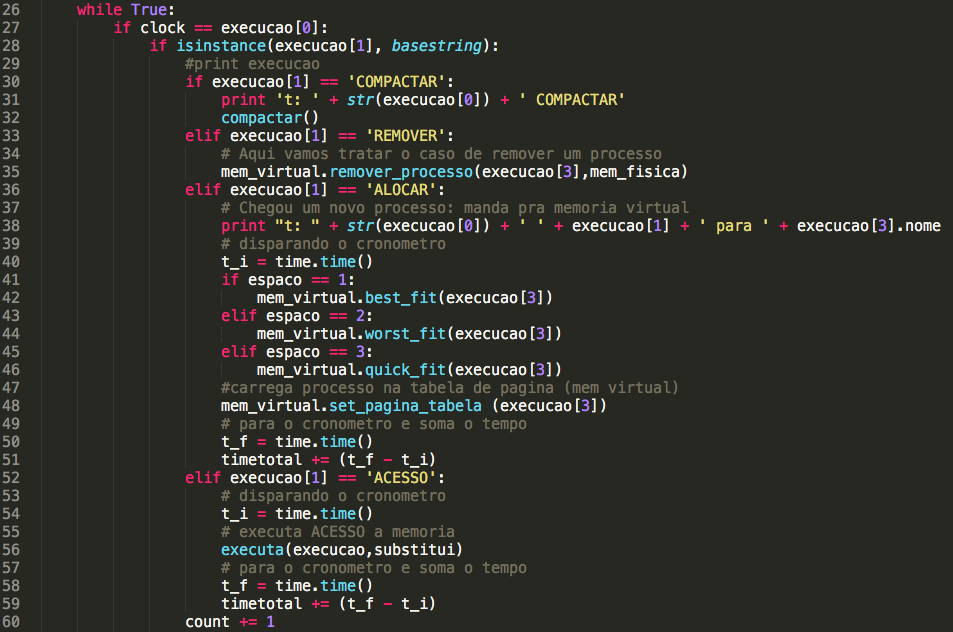
\includegraphics[width=0.8\textwidth]{fig/loop_simula.png}
\caption{Trecho com o \textit{loop} da simulação.}
\label{fig:loop}
\end{figure}


\item \textbf{linkedlist.py}: Nesse modulo está implementado a classe que vai criar e manipular a lista encadeada. Os nós da lista são da seguinte forma:
\begin{lstlisting}
class Node(object):
    def __init__(self, data, inicio, tamanho, next_node):
        self.data = data                # L se eh um noh livre e P se tem processo
        self.inicio = int(inicio)       # Em que posicao comeca
        self.tamanho = int(tamanho)     # Tamanho ocupado
        self.next_node = next_node      # Proximo noh
        self.previous_node = None       # No anterior
\end{lstlisting}
O objetivo dessa classe é guardar os espaços livres e ocupados a memoria. 

\begin{figure}[htpb]
\centering
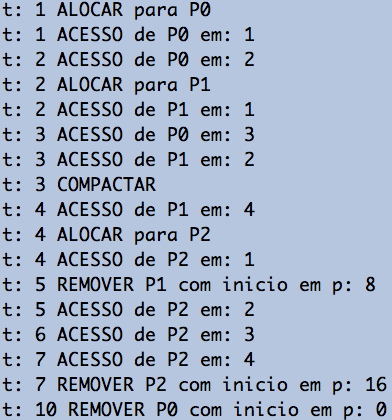
\includegraphics[width=0.3\textwidth]{fig/lista_execucao.png}
\caption{Exemplo de uma lista de execução ordenada em ordem crescente de tempo \texttt{t}.}
\label{fig:execucao}
\end{figure}

\item \textbf{memory.py}: Nesse modulo estão todas as implementações referentes à memoria. Temos uma classe Memory:
\begin{lstlisting}
class Memory:
    def __init__ (self, total, s, p, filename):
    
        self.tamanho = total
        self.s = s
        self.p = p
        self.arquivo = filename
        self.tabela = []
        #monta a tabela de paginas para esta memoria
        self.set_tabela()
        #lista que vai espelhar a situacao da memoria. Vamos escrever essa lista no arquivo
        self.vetor = [-1] * self.tamanho 
        #lista ligada para controle do espaco livre da memoria
        self.lista = LinkedList('L',0,self.tamanho,None)
        #Abre o arquivo para a memoria
        self.memfile = open (filename,'wb')
        #define tamanho do arquivo binario em bytes
        # b signed char => 1 byte
        self.memfile.write(pack(str(self.tamanho)+'b',*self.vetor))
        self.memfile.flush()
\end{lstlisting}

É aqui também que estão implementados os algoritmos de gerência de memórias, que serão detalhados mais a frente.

\item \textbf{paging.py}: Aqui estão os algoritmos de substituição de páginas e também temos uma classe Page:
\begin{lstlisting}
#classe page: representa uma pagina na tabela de paginas
class Page:
    def __init__ (self, inicio, p):
        self.tamanho = p                 #define o tamanho da pagina
        self.inicio = int(inicio)        #onde a pagina comeca
        self.fim = int(inicio) + p - 1   #onde a pagina termina
        self.presente = 0                #presente = 1 se a pagina esta mapeada na memoria fisica e 0 caso contrario
        self.mapeada = -1                #link recebe o indice da pagina que esta linkada na memoria fisica
        self.procId = -1                 #O id do processo dono desta pagina
        self.tAcesso = -1
        self.m = 0
        self.r = 0
        self.countLRUv4 = 0  
\end{lstlisting}

\item \textbf{processo.py}: Nesse modulo temos a classe processo e seus métodos para lidar com suas variáveis. 
\begin{lstlisting}
class Processo:
    current_pid = 0

    def __init__(self, t0, tf, b, nome, acessos):
        self.t0 = int(t0)         # tempo de chegada do processo
        self.tf = int(tf)         # tempo de termino do processo
        self.b = int(b)           # tamanho de memoria requisitado pelo processo
        self.nome = nome          # string com nome do processo
        self.ocupa = 0            # tamanho ocupado pelo processo devido a uniadade de alocacao (tamanho marcado com seu pid)
        self.reserva = 0          # tamanho reservado pelo processo devida ao tamanho da pagina  
        self.base = -1            # endereco base do processo
        self.limite = -1          # endereco limite do processo  
        self.setpid()             # define pid do processo
        self.setAcessos(acessos)  # pares de acesso a memoria (pn,tn)

\end{lstlisting}

\item \textbf{run\_tests.sh}: Shell-script que gera os resultados para todas as combinações de algoritmos de espaço e substituição.
\end{itemize}

A seguir são descritas as implementações dos algoritmos de gerência de espaço livre e dos algoritmos de substituição de páginas. Todas as implementações foram feitas com base nas notas de aulas e com referências de \cite{tanenbaum2009m}.

Algumas considerações gerais sobre a implementação são comentadas a seguir:

\begin{itemize}
\item Quando duas ações (alocação de memoria na chegada de um processo, acesso a uma posição, etc.) acontecem no mesmo instante de tempo, é mantido a ordem em que a ação aparece no trace;
\item o \texttt{clock} (que conta o tempo na simulação) é um contador que incrementa em um \textit{loop};
\item os tamanhos das memórias são em \textit{bytes}, cada \textit{byte} representa uma posição da memória;
\item para a conversão dos bytes foi utilizados as funções \texttt{pack} e \texttt{unpack} da biblioteca \texttt{struct} do Python.

\item os tempos de busca de espaço livre foram feitos com a função \texttt{time()} da biblioteca \texttt{time} em trechos do código em que eram aplicados os algoritmos gerência de memória.

\end{itemize}

\subsection{Algoritmos de gerência de espaço livre}

Os algoritmos se baseiam na lista ligada para gerência de espaço livre da memória virtual.
Assumimos para estes algoritmos que sempre existirá espaço na memória virtual para quaisquer processos que cheguem para execução.
Cada nó da lista ligada para a gerência de espaço livre tem a configuração como descrita acima  em \textit{class Node(object)}

\subsubsection{Best-Fit}
\begin{lstlisting}
def best_fit(self, p):
\end{lstlisting}
Este algoritmo é implementado como procedimento da classe Memory. Ele recebe um processo \textit{p} e varre toda a lista de controle de espaço livre da memória virtual em busca do espaço livre que tenha o menor tamanho suficiente para acomodar todo o processo, levando em consideração o número de páginas que o processo em questão deve ocupar.
Quando este processo é alocado, definem-se as posições \textit{base} e \textit{limite} para o mesmo.

\subsubsection{Worst-Fit}	
\begin{lstlisting}
def worst_fit(self, p):
\end{lstlisting}
Análogo \textit{Best-Fit}este algoritmo é também implementado como procedimento da classe Memory. Ele recebe um processo \textit{p} e varre toda a lista ligada de controle de espaço livre da memória virtual em busca do espaço livre que tenha o maior tamanho para acomodar o processo. Com base na posição alocada, defini-se a \textit{base} e \textit{limite} para o processo.

\subsubsection{Quick-Fit}
\begin{lstlisting}
def quick_fit(self, p):
\end{lstlisting}
A ideia deste algoritmo é criar listas que mapeiem os 3 espaços de alocação mais requisitados pelo processos. Não conseguimos terminar a implementação deste algoritmo.


\subsection{Algoritmos de substituição de páginas}
A nossa implementação da parte de substituição de paginas ocorre sempre depois olhar toda a tabela de paginas da memoria física e verificar que não há um espaço para alocar uma nova página. Se houver um lugar, a nova página ocupa esse espaço. Caso contrário, entram os algoritmos de substituição de páginas para escolher qual página será retirada da memória física. Quando o código usa algoritmo de substituição além de escolher a página que vai ser removida é preciso fazer todo o remapeamento das tabelas de páginas e marcar (de acordo com as especificidades de cada algoritmo) a nova pagina que entrou na memória. O ideia do código de remapeamento de tabelas é comum a todos os algoritmos de substituição. 

A seguir são apresentados alguns detalhes das implementações dos algoritmos de substituição de página. 
\subsubsection{Optimal}
Não conseguimos terminar a implementação desse algoritmo a tempo.
\subsubsection{First in, First Out}
Toda vez que uma página é mapeada na memória é guardado na página o \texttt{clock}, no qual ela entrou na memória. Usa-se esse valor para descobrir qual é a pagina mais velha e com isso remove-se página que foi mapeada a mais tempo.
\subsubsection{Least Recently Used (Segunda Versão)}
A implementação procurou ser fiel ao algoritmo apresentado em sala de aula, no qual utiliza-se uma matriz quadrada de tamanho igual ao numero de paginas que cabe na memória. Toda vez que uma pagina é mapeada ou acessada na memória física marca-se a linha e em seguida a coluna matriz correspondente a posição da pagina. Quando ocorre um Pagefault, busca-se nessa matriz a pagina que foi menos referenciada.
\begin{lstlisting}
# devolve a pagina menos acessada de acordo com a matriz de acesso matriz_LRUv2
def LRUv2_pagina (npaginas):
    global matriz_LRUv2
    maior = int(''.join(npaginas*['1']),2) 
    pagina = 0
    for i in range(npaginas):
        x = int(''.join(matriz_LRUv2[i]),2) # converte a linha binaria para int
        if x < maior:
            pagina = i 
            maior = x
    return pagina
\end{lstlisting}

\subsubsection{Least Recently Used (Quarta Versão)}
Na implementação do LRUv4 nós usamos uma variável extra da nossa classe Pagina :
\begin{lstlisting}
self.countLRUv4 = 0  
\end{lstlisting}

que é atualizada a cada acesso ou mapeamento com o seguinte método:
\begin{lstlisting}
def set_countLRUv4(self,k):
        self.countLRUv4 += 1
        self.countLRUv4 =  self.countLRUv4%k
\end{lstlisting}

Basicamente, a variável \texttt{k} vai definir a "idade" máxima da página, equivalente ao número de bits, da implementação apresentada em classe. Quando ocorre um Pagefault, retira-se a página com o menor \texttt{countLRUv4}. O valor \texttt{k} foi fixado em $k=6$ em todo nosso código.

\section{Resultados}

Para gerar os resultados aqui apresentados foi utilizado um \textit{Shell-script} (\texttt{run\_tests.sh}) para gerar 30 execuções em modo \textit{batch} de um trace. Em toda execução o \texttt{ep3.py} sempre vai imprimir o tempo total que levou para fazer todas as buscas por um espaço livre na memória durante uma simulação e o número de ocorrências de \textit{PageFaults}. Esse script pode ser executado para qualquer trace, com a seguinte chamada:

\begin{lstlisting}
$ ./run_tests.sh trace.txt
\end{lstlisting}

Um exemplo de saída do script para um arquivo \textit{trace} qualquer é mostrado na Figura \ref{fig:run_tests}. A média e o desvio padrão foram calculados usando o \texttt{awk}.
\begin{lstlisting}
media_std=$(
    for i in  ${results}; do echo $i;done |
        awk '{sum+=$1; sumsq+=$1*$1}END{print sum/NR " " sqrt(sumsq/NR - (sum/NR)**2)}'
)
\end{lstlisting}
\begin{figure}[htpb]
\centering
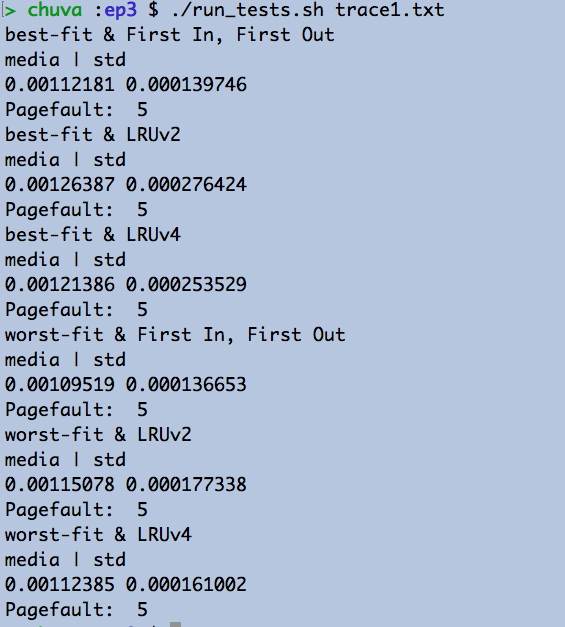
\includegraphics[width=0.4\textwidth]{fig/run_tests.png}
\caption{Média e desvio padrão de 30 execuções de um arquivo \textit{trace} para a combinação de todos os algoritmos de gerência de espaço com os algoritmos de substituição de paginas implementados.}
\label{fig:run_tests}
\end{figure}

\begin{figure}[htpb]
\centering
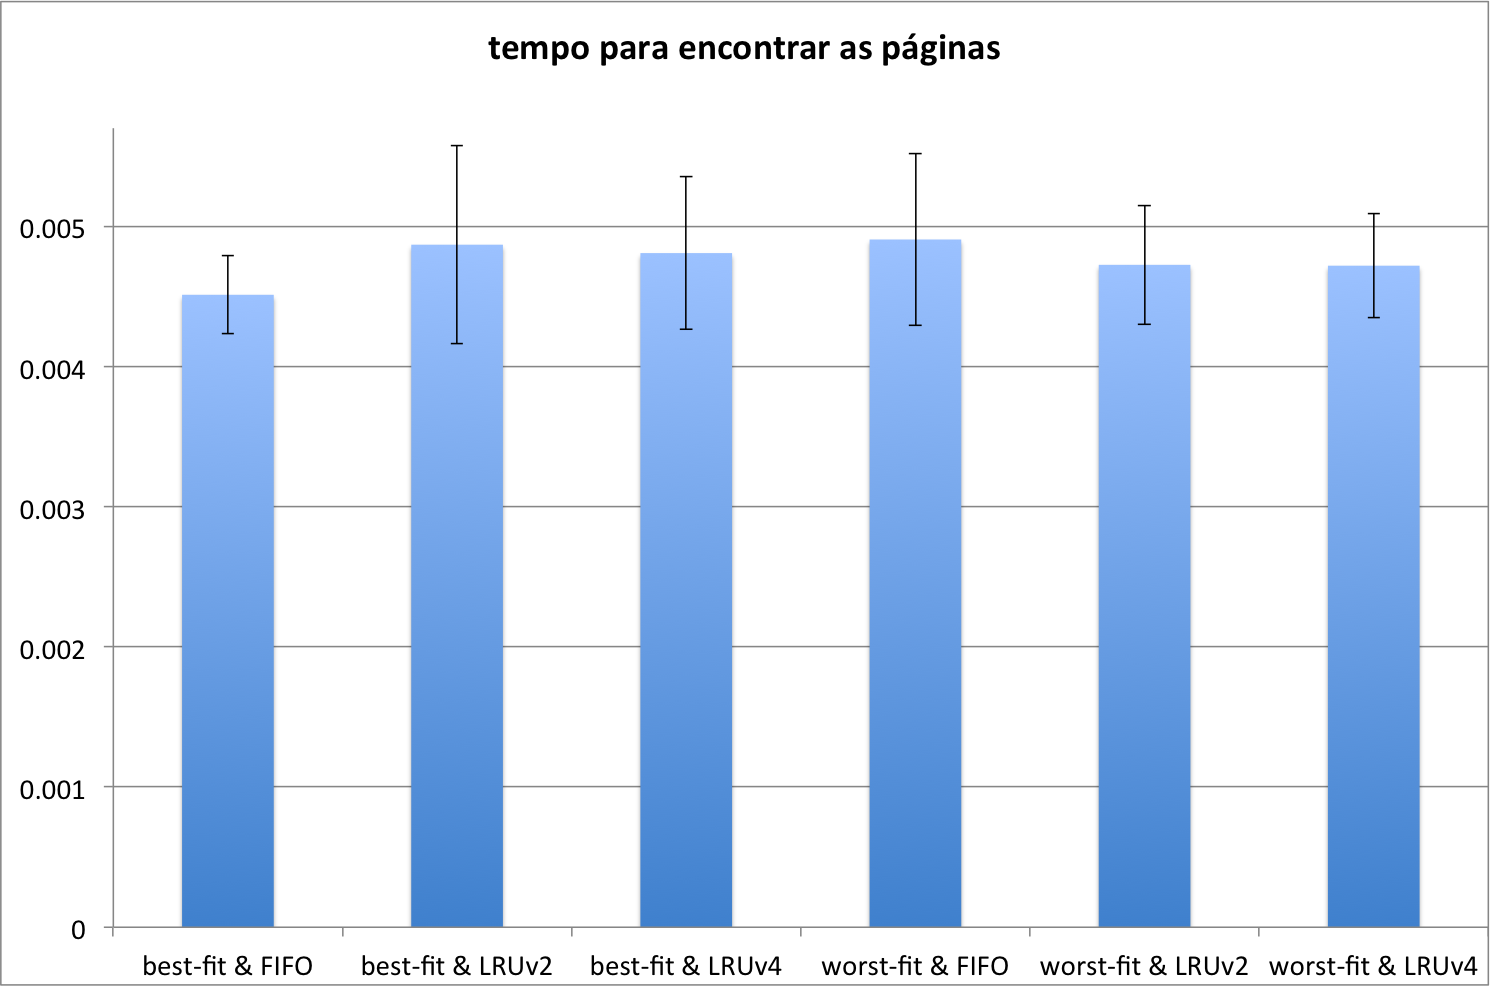
\includegraphics[width=0.8\textwidth]{fig/resultados_ep3.png}
\caption{Média e desvio padrão de 30 execuções de um arquivo \textit{trace} para a combinação de todos os algoritmos de gerência de espaço com os algoritmos de substituição de paginas implementados.}
\label{fig:tempo}
\end{figure}

A Figura \ref{fig:tempo} resume todos os testes feitos com os algoritmos implementados. Nessa figura são apresentados a média e o desvio padrão de 30 simulações de um arquivo trace teste. Esse \textit{trace} foi produzido com intuito de tentar evidenciar algumas características dos algoritmos. Cada barra da Figura \ref{fig:tempo} representa uma combinação de um algoritmo de gerência de espaço com um algoritmo de substituição de página. 

A Figura \ref{fig:pagefault} mostra as ocorrências de Pagefaults para o arquivo trace testado. A quantidade de Pagefault não vai variar pra diferentes rodadas de um mesmo trace. Dessa forma, os resultados desse análise não possuem o desvio padrão.

Os resultados mostrados nas Figuras \ref{fig:tempo} e \ref{fig:pagefault} não conseguiram evidenciar forma muito clara as diferenças de comportamento entre as combinações de algoritmos. Acredita-se que um dos motivos principais para tal comportamento tenha sido a presença de alguma operação "gargalo" que tenha sido feita no trecho de codigo que tentamos cronometrar o tempo de busca de página. Como as implementações dos algoritmos \texttt{quick-fit} e \textit{Optimal} não conseguiram ficar prontas a tempo de confeccionar os resultados, não mostramos os resultados com essas combinações. E muito provavelmente seria possível ver ganhos de tempo com o uso desses algoritmos.  

\begin{figure}[htpb]
\centering
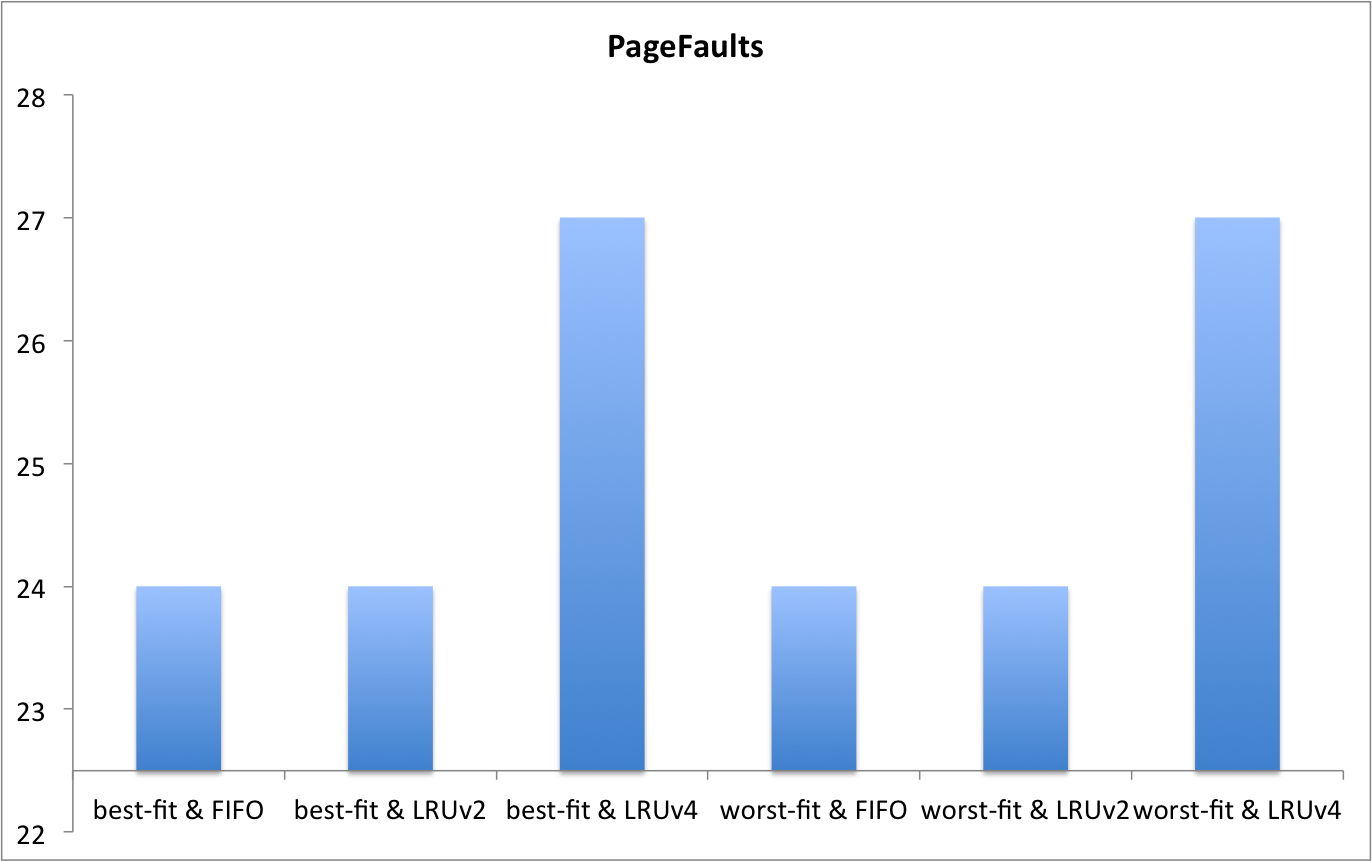
\includegraphics[width=0.8\textwidth]{fig/pagefault_ep3.png}
\caption{Quantidade de Pagefaults para todas as combinações dos algoritmos de gerência de espaço com os algoritmos de substituição de paginas implementados.}
\label{fig:pagefault}
\end{figure}

\section{Divisão das tarefas de implementação}

O repositório no qual foi desenvolvido o projeto encontra-se em \url{https://github.com/rasouza/ep3-so/}. Algumas informações dos \textit{logs} do repositório (\texttt{commits} e linhas adicionadas) são mostradas a seguir:

\begin{lstlisting}
$ git shortlog -sn
    41  brferrero
    30  taispin
     3  Rodrigo Alves
     3  Tais
$ git log --author="<USER>" --pretty=tformat: --numstat | awk '{inserted+=$1} END {printf "Commit stats:\n- Lines added (total)....  %s\n", inserted}'
USER=brferrero (Bruno Ferrero)
Commit stats:
- Lines added (total)....  802
USER=Rodrigo Alves
Commit stats:
- Lines added (total)....  167
USER=taispin (Tais Pinheiro)
Commit stats:
- Lines added (total)....  739
\end{lstlisting}

A participação no início do projeto foi bastante intensa por parte de todos os membros do grupo. Houve bastante discussão para podermos entender o que deveria ser implementado e como. Ao final do projeto foi possível notar que grande parte das decisões de projeto tomadas de início foram respeitadas e acertadas.

\bibliography{biblio.bib}
\bibliographystyle{./elsart-harv}
\end{document}